\section{Toy Experiments}
The first toy experiment uses two identical outputs which are noisy version of the same version plus some noise: $y_1(x) = sin(x) + \epsilon$ and $y_2(x) = sin(x) + \epsilon$, $\epsilon \sim \Normal(0,0.01)$.
In this case the shared function $g(x)$ is $sin(x)$ and the independent processes $h_1(x)$ and $h_2(x)$ are just white noises.
Each output has missing values in one region of the input space.
The predictive distributions of the multiple-gp model compared to that of independent gps are shown in \ref{fig4}.

\noindent The second toy experiment uses similar setting as the first one, except that now $y_1(x) = sin(x) + \epsilon$ and $y_2(x) = -sin(x) + \epsilon$. 
In this case the shared function is still $g(x) = sin(x)$, but the weights should be opposite i.e. $w_1 = 1$ and $w_2 = 1$.
The learning procedure was indeed able to recovered this relation and learned that $w_1 = 1.2$ and $w_2 = -1.3$.
The predictive distributions are shown in \ref{fig5}.

\begin{figure*}
\centering
\begin{tabular}{cc}
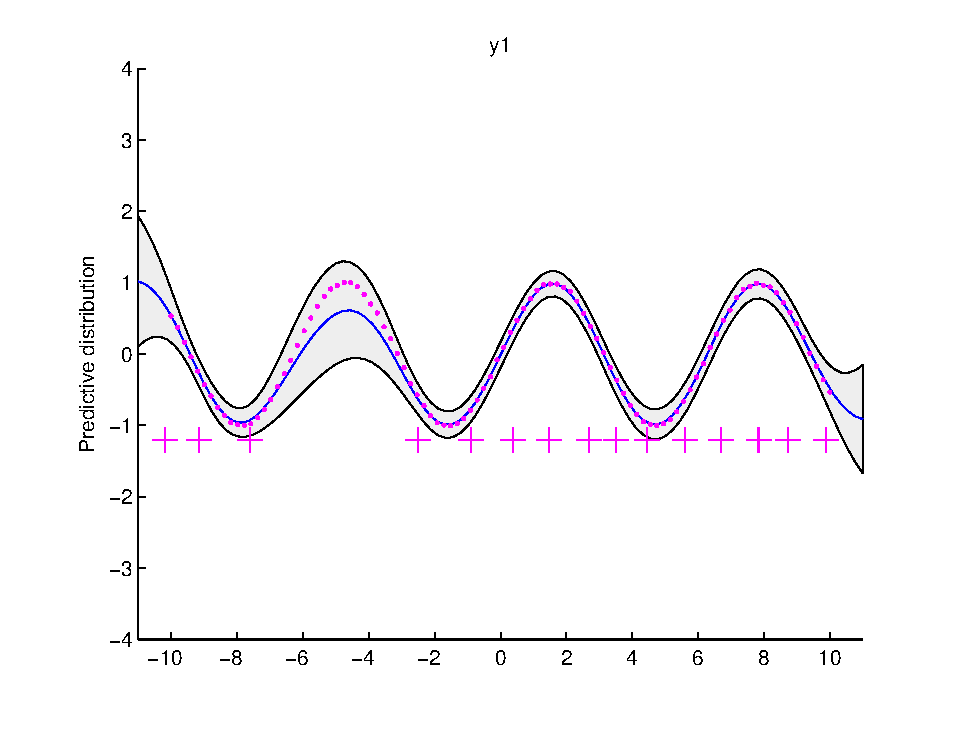
\includegraphics[scale=0.5]{figures/ssvi-y1.eps} &
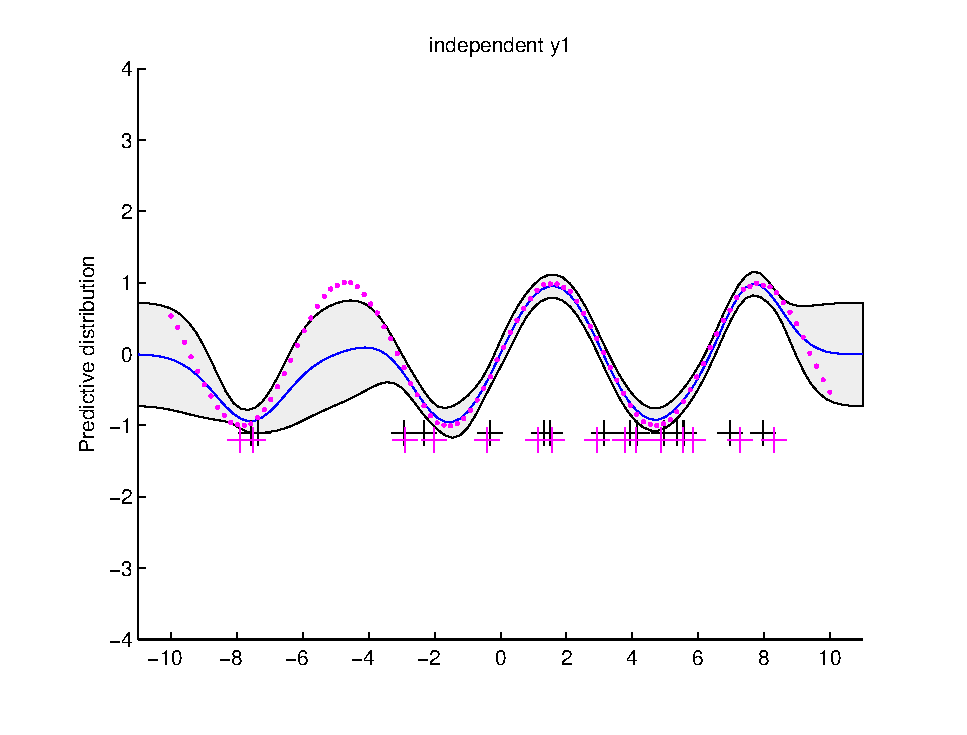
\includegraphics[scale=0.5]{figures/ssvi-svi1.eps} \\
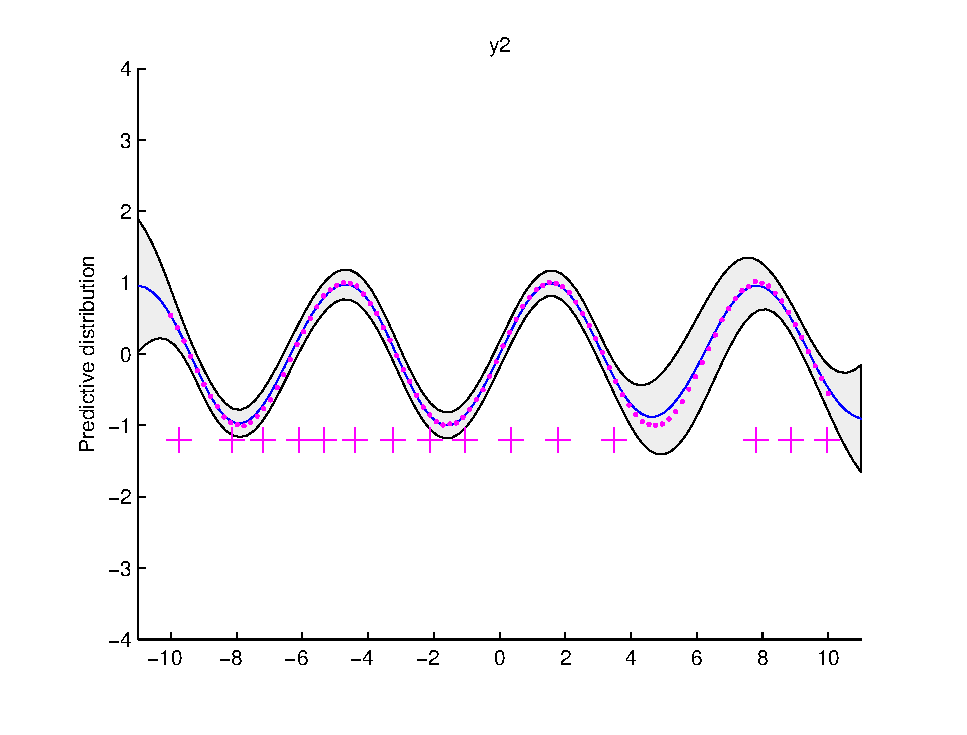
\includegraphics[scale=0.5]{figures/ssvi-y2.eps} &
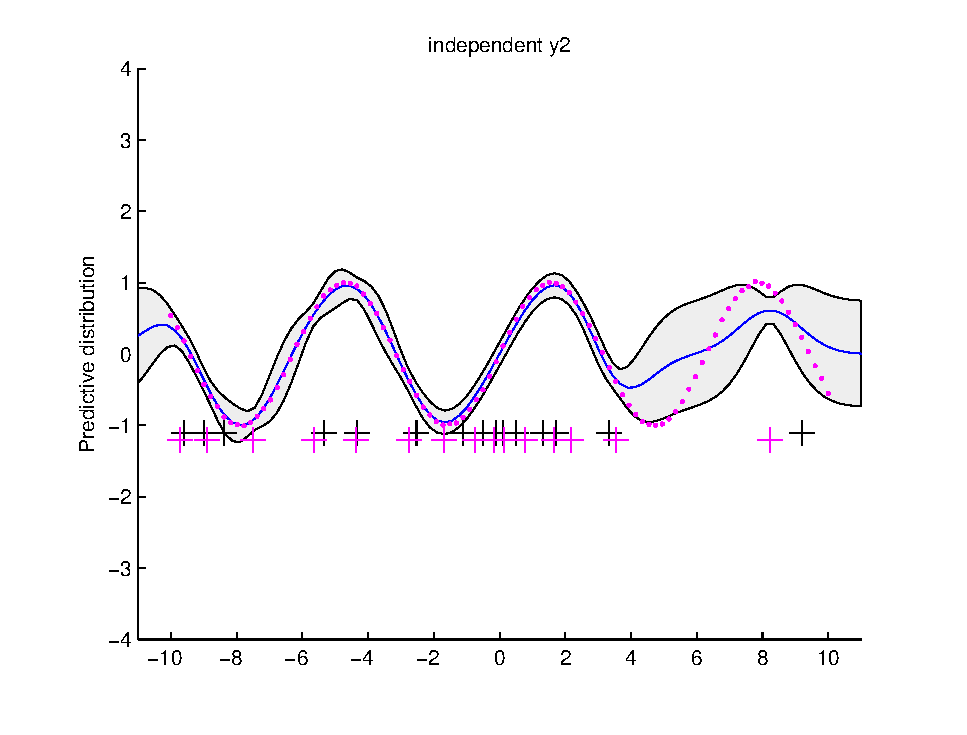
\includegraphics[scale=0.5]{figures/ssvi-svi2.eps} \\
\multicolumn{2}{c}{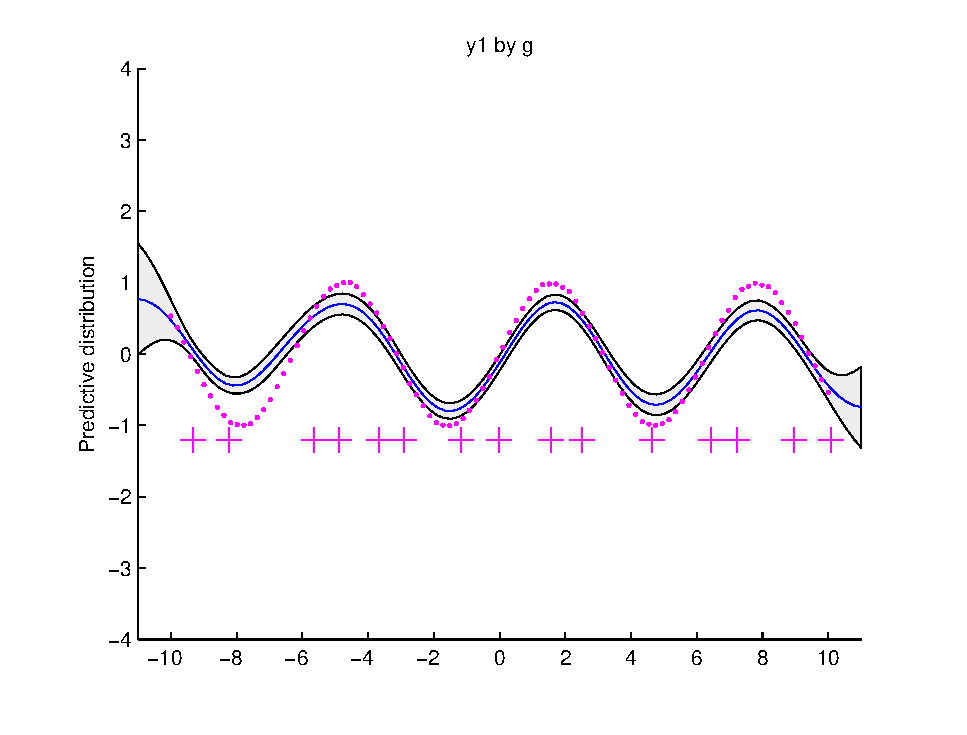
\includegraphics[scale=0.5]{figures/ssvi-y1byg.eps} }
\end{tabular}
\label{fig4}
\caption{Predictive distributions of the multipe-output gps (left column) and independent gps (right column) for the first toy example. The predictive distribution by $g(x)$ for $y_1(x)$ is shown in the bottom figure.}
\end{figure*}

\begin{figure*}
\centering
\begin{tabular}{cc}
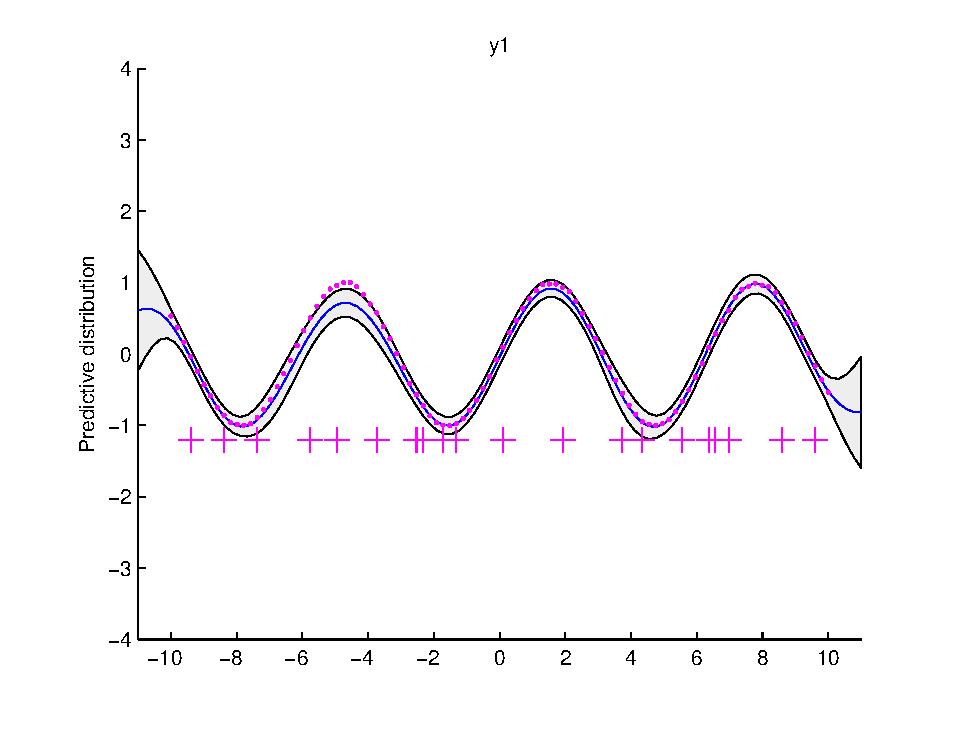
\includegraphics[scale=0.5]{figures/ssvi2-y1.eps} &
\includegraphics[scale=0.5]{figures/ssvi2-svi1.eps} \\
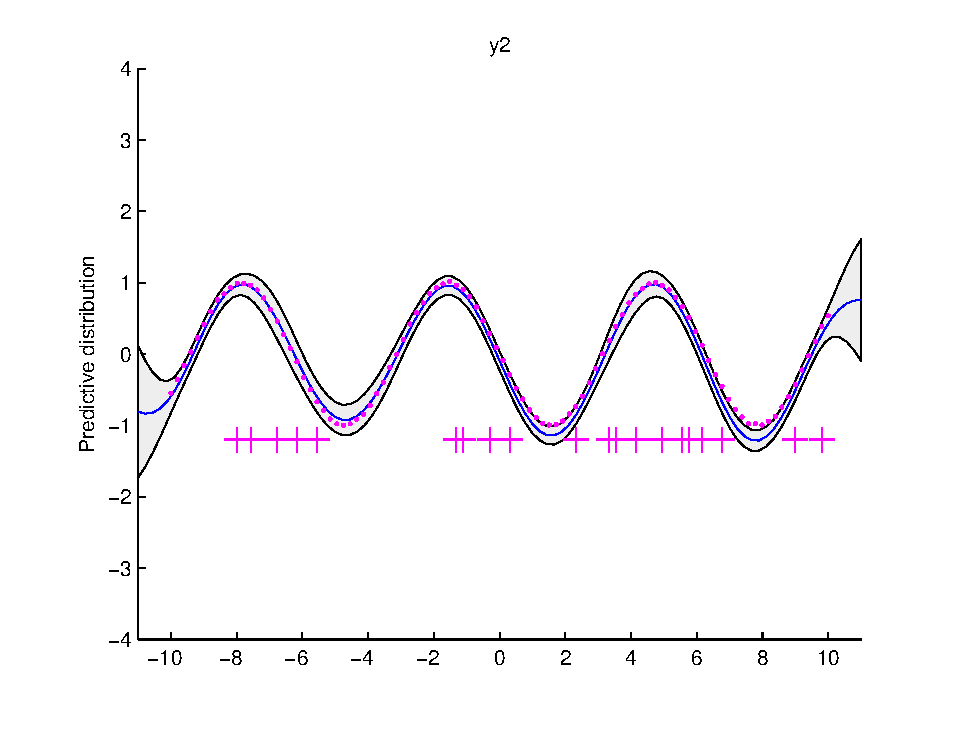
\includegraphics[scale=0.5]{figures/ssvi2-y2.eps} &
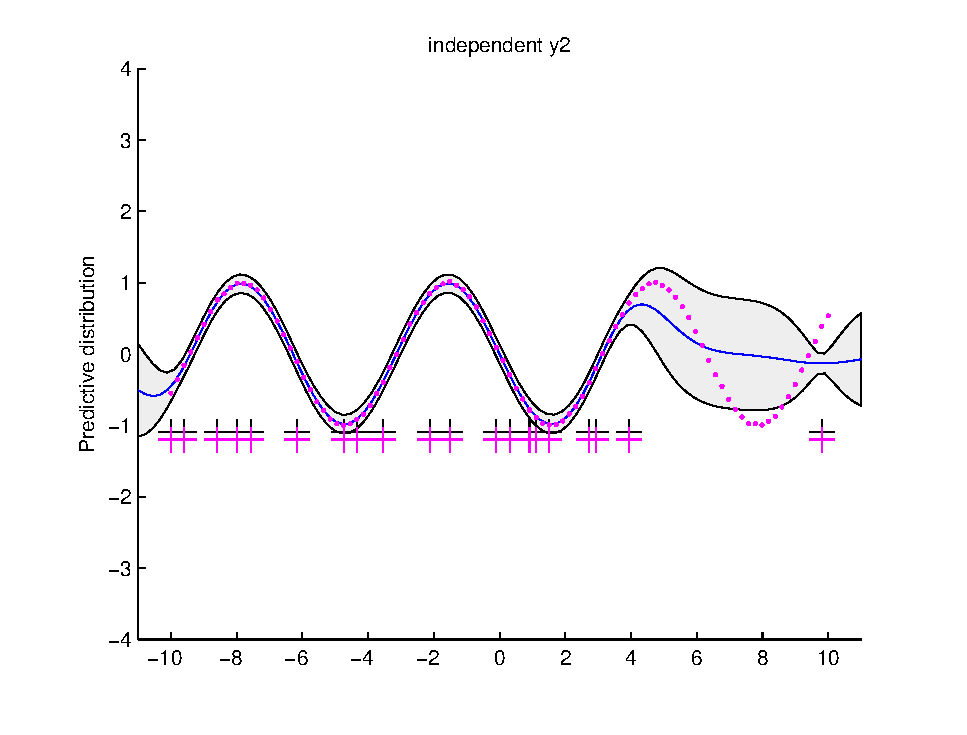
\includegraphics[scale=0.5]{figures/ssvi2-svi2.eps} \\
\multicolumn{2}{c}{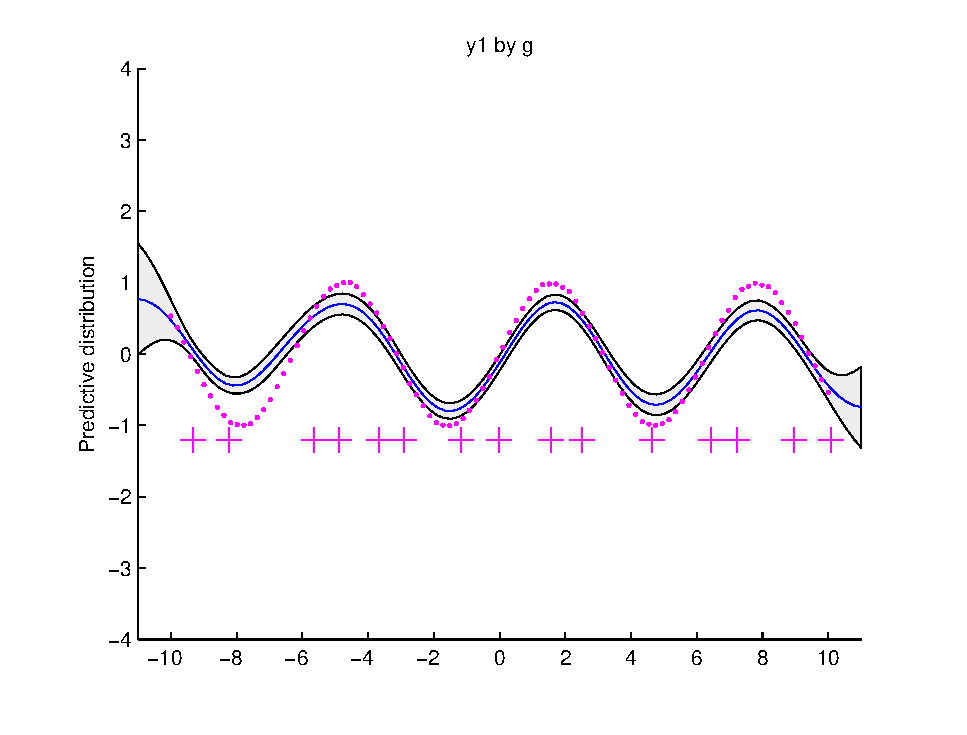
\includegraphics[scale=0.5]{figures/ssvi-y1byg.eps} }
\end{tabular}
\label{fig5}
\caption{Predictive distributions of the multipe-output gps (left column) and independent gps (right column) for the second toy experiment. The predictive distribution by $g(x)$ for $y_1(x)$ is shown in the bottom figure.}
\end{figure*}

